\section{Diseño de la Base de Datos}
\label{sec:diseno_bd}

En este apartado se explica cómo se guarda y se organiza la información dentro de la página web usando una base de datos relacional \parencite{silberschatz2014}. Toda la información se reparte en tablas conectadas entre sí para que nada se pierda ni se revuelva, asegurando que las cuentas funcionen bien, los archivos en PDF se guarden por versiones sin borrar nada viejo, las reuniones queden registradas con sus tareas y el sistema avise si alguien pasa más de un mes sin trabajar \parencite{sim2023technology}.

\subsection{Descripción del Proyecto y Elementos de la Base de Datos}
\label{subsec:descripcion_bd}

Para entender el diagrama del sistema, la información se organiza en tres cosas muy sencillas: las tablas principales que representan a los elementos del sistema (rectángulos), los datos específicos que guarda cada una (óvalos o bolitas) y las conexiones que explican cómo se relacionan entre sí (rombos) \parencite{silberschatz2014}.

\subsubsection{Tablas y qué datos guarda cada una}

La base de datos empieza con la tabla llamada \textit{usuario}, que sirve para controlar el acceso de todas las personas a la página web. Esta tabla utiliza como dato principal el \underline{id\_usuario}, que es un número único para cada cuenta que no se repite. Además, guarda datos básicos como el \textit{correo\_institucional} para iniciar sesión, la \textit{contrasena}, la \textit{fecha\_registro} y la casilla de \textit{cuenta\_activa} para saber si la persona puede entrar o está dada de baja. El nombre de la persona se guarda en un dato llamado \textit{nombre\_completo}, el cual se divide en primer nombre, segundo nombre, apellido paterno y apellido materno para que sea fácil ordenar las listas por orden alfabético. También incluye el dato de \textit{telefono}, que se dibuja con doble óvalo porque una persona puede registrar más de un número para que la localicen. Como no todos hacen lo mismo en la página web, esta cuenta general se divide en tres tipos de usuario: el \textit{alumno}, que guarda su matrícula escolar; el \textit{asesor}, que guarda su número de maestro y su grado de estudios; y el \textit{coordinador}, que guarda el número de su oficina y su teléfono de atención.

La siguiente tabla es \textit{proyecto\_tesis}, que funciona como el expediente principal del trabajo de investigación. Tiene su propio identificador llamado \underline{id\_proyecto} y guarda datos como el \textit{titulo\_tesis}, el tema o \textit{linea\_investigacion}, la \textit{fecha\_inicio}, la \textit{fecha\_ultimo\_avance} y cómo va el trabajo en el \textit{estado\_proyecto}. En esta tabla se incluye un dato especial llamado \textit{dias\_inactividad}, que en el dibujo lleva una bolita con línea punteada porque nadie lo escribe a mano; la página web hace una resta automática entre la fecha de hoy y la fecha del último avance para saber cuántos días lleva el alumno sin entregar nada.

Para guardar los documentos del estudiante se utiliza la tabla \textit{entregable\_version}. En el dibujo se coloca con un rectángulo doble porque es una tabla dependiente; es decir, no tiene sentido guardar un archivo suelto si no pertenece a una tesis ya registrada. Esta tabla usa el dato \underline{numero\_version} para enumerar las entregas (como versión 1, versión 2 o versión 3), logrando que cada trabajo nuevo se guarde por separado sin borrar los archivos anteriores. También guarda la \textit{ruta\_archivo\_pdf} donde quedó el documento, la \textit{fecha\_hora\_subida}, una nota escrita por el estudiante en \textit{comentario\_alumno} y las correcciones que le escribe el maestro en \textit{retroalimentacion\_asesor}.

Para llevar el control de las citas de asesoría se tiene la tabla \textit{minutas\_asesoria}, que se identifica con el número \underline{id\_minuta}. Aquí se guarda la \textit{fecha\_reunion}, si la cita fue en persona o por internet en \textit{modalidad}, un resumen de lo que platicaron en \textit{resumen\_temas} y el día en que se capturó la información en \textit{fecha\_registro}.

Pegada a cada minuta se encuentra la tabla \textit{compromiso\_acuerdo}, que también se dibuja con recuadro doble porque las tareas solo existen si se acordaron en una reunión previa. Se organiza mediante el número de tarea \underline{numero\_acuerdo} y guarda qué hay que hacer en \textit{descripcion\_tarea}, a quién le toca cumplirla en \textit{responsable} (si al alumno o al maestro), el día máximo de entrega en \textit{fecha\_limite} y una casilla de \textit{estado\_cumplido} para marcar si ya se entregó o si sigue pendiente.

Por último, se encuentra la tabla \textit{alerta\_rezago}, que se encarga de guardar los avisos automáticos que manda la página web. Cuenta con su número de aviso \underline{id\_alerta} y guarda el día del aviso en \textit{fecha\_deteccion}, cuántos días sin avance se contaron en \textit{dias\_acumulados} y si el aviso ya fue atendido por el profesor en \textit{estado\_alerta}.

\subsubsection{Cómo se conectan las tablas y cuántos datos abarcan (Cardinalidades)}

Las líneas y los rombos del dibujo muestran cómo se comunica una tabla con otra y cuántos registros puede tener cada conexión. La tabla general de \textit{usuario} se conecta con cada tipo de cuenta (\textit{alumno}, \textit{asesor} y \textit{coordinador}) mediante una relación de uno a uno ($1:1$), lo que significa que cada cuenta de la página web le pertenece exactamente a una sola persona con su perfil correspondiente.

A partir de ahí, el \textit{alumno} se une con \textit{proyecto\_tesis} mediante la acción Desarrolla con una relación de uno a uno ($1:1$). Esto indica que un estudiante solo puede tener una tesis activa en la página web y que cada tesis le pertenece a un solo alumno. En cambio, el \textit{asesor} se conecta con \textit{proyecto\_tesis} con la acción Dirige en una relación de uno a muchos ($1:N$), porque un profesor puede asesorar a varios alumnos al mismo tiempo, pero cada trabajo de tesis tiene a un solo maestro titular a cargo. Por su parte, el \textit{coordinador} se conecta con la tesis mediante la acción Supervisa ($1:N$), ya que la coordinación tiene permiso de entrar a revisar todos los proyectos registrados en la escuela sin ser el director directo de ninguno de ellos.

En cuanto al manejo de los trabajos y documentos, la tabla \textit{proyecto\_tesis} se conecta con \textit{entregable\_version} a través del rombo doble Guarda versiones ($1:N$). Esto significa que a lo largo de los meses una tesis va juntando muchos borradores en PDF, pero cada archivo pertenece estrictamente a ese trabajo. De la misma forma, el proyecto se conecta con \textit{minutas\_asesoria} mediante la acción Registra ($1:N$), acumulando todas las juntas que se realicen durante el posgrado. Cada minuta se conecta a su vez con la tabla dependiente \textit{compromiso\_acuerdo} mediante el rombo doble Contiene tareas ($1:N$), lo que asegura que de cada reunión salgan una o varias tareas obligatorias por cumplir. Para terminar, la tesis se conecta con \textit{alerta\_rezago} con la acción Dispara aviso ($1:N$), lo que permite que el sistema guarde una alerta cada vez que el reloj automático note que el estudiante lleva más de 30 días seguidos sin registrar avances ni minutas.

\clearpage

\subsection{Diagrama Entidad--Relación}
\label{subsec:diagrama_eer}

En la Figura~\ref{fig:diagrama_eer} se muestra el dibujo completo de la base de datos, donde se aprecian las tablas normales, las tablas dependientes con doble línea, los datos con sus diferentes tipos de bolitas y los números que indican cómo se unen entre sí.

\begin{figure}[htbp]
    \centering
    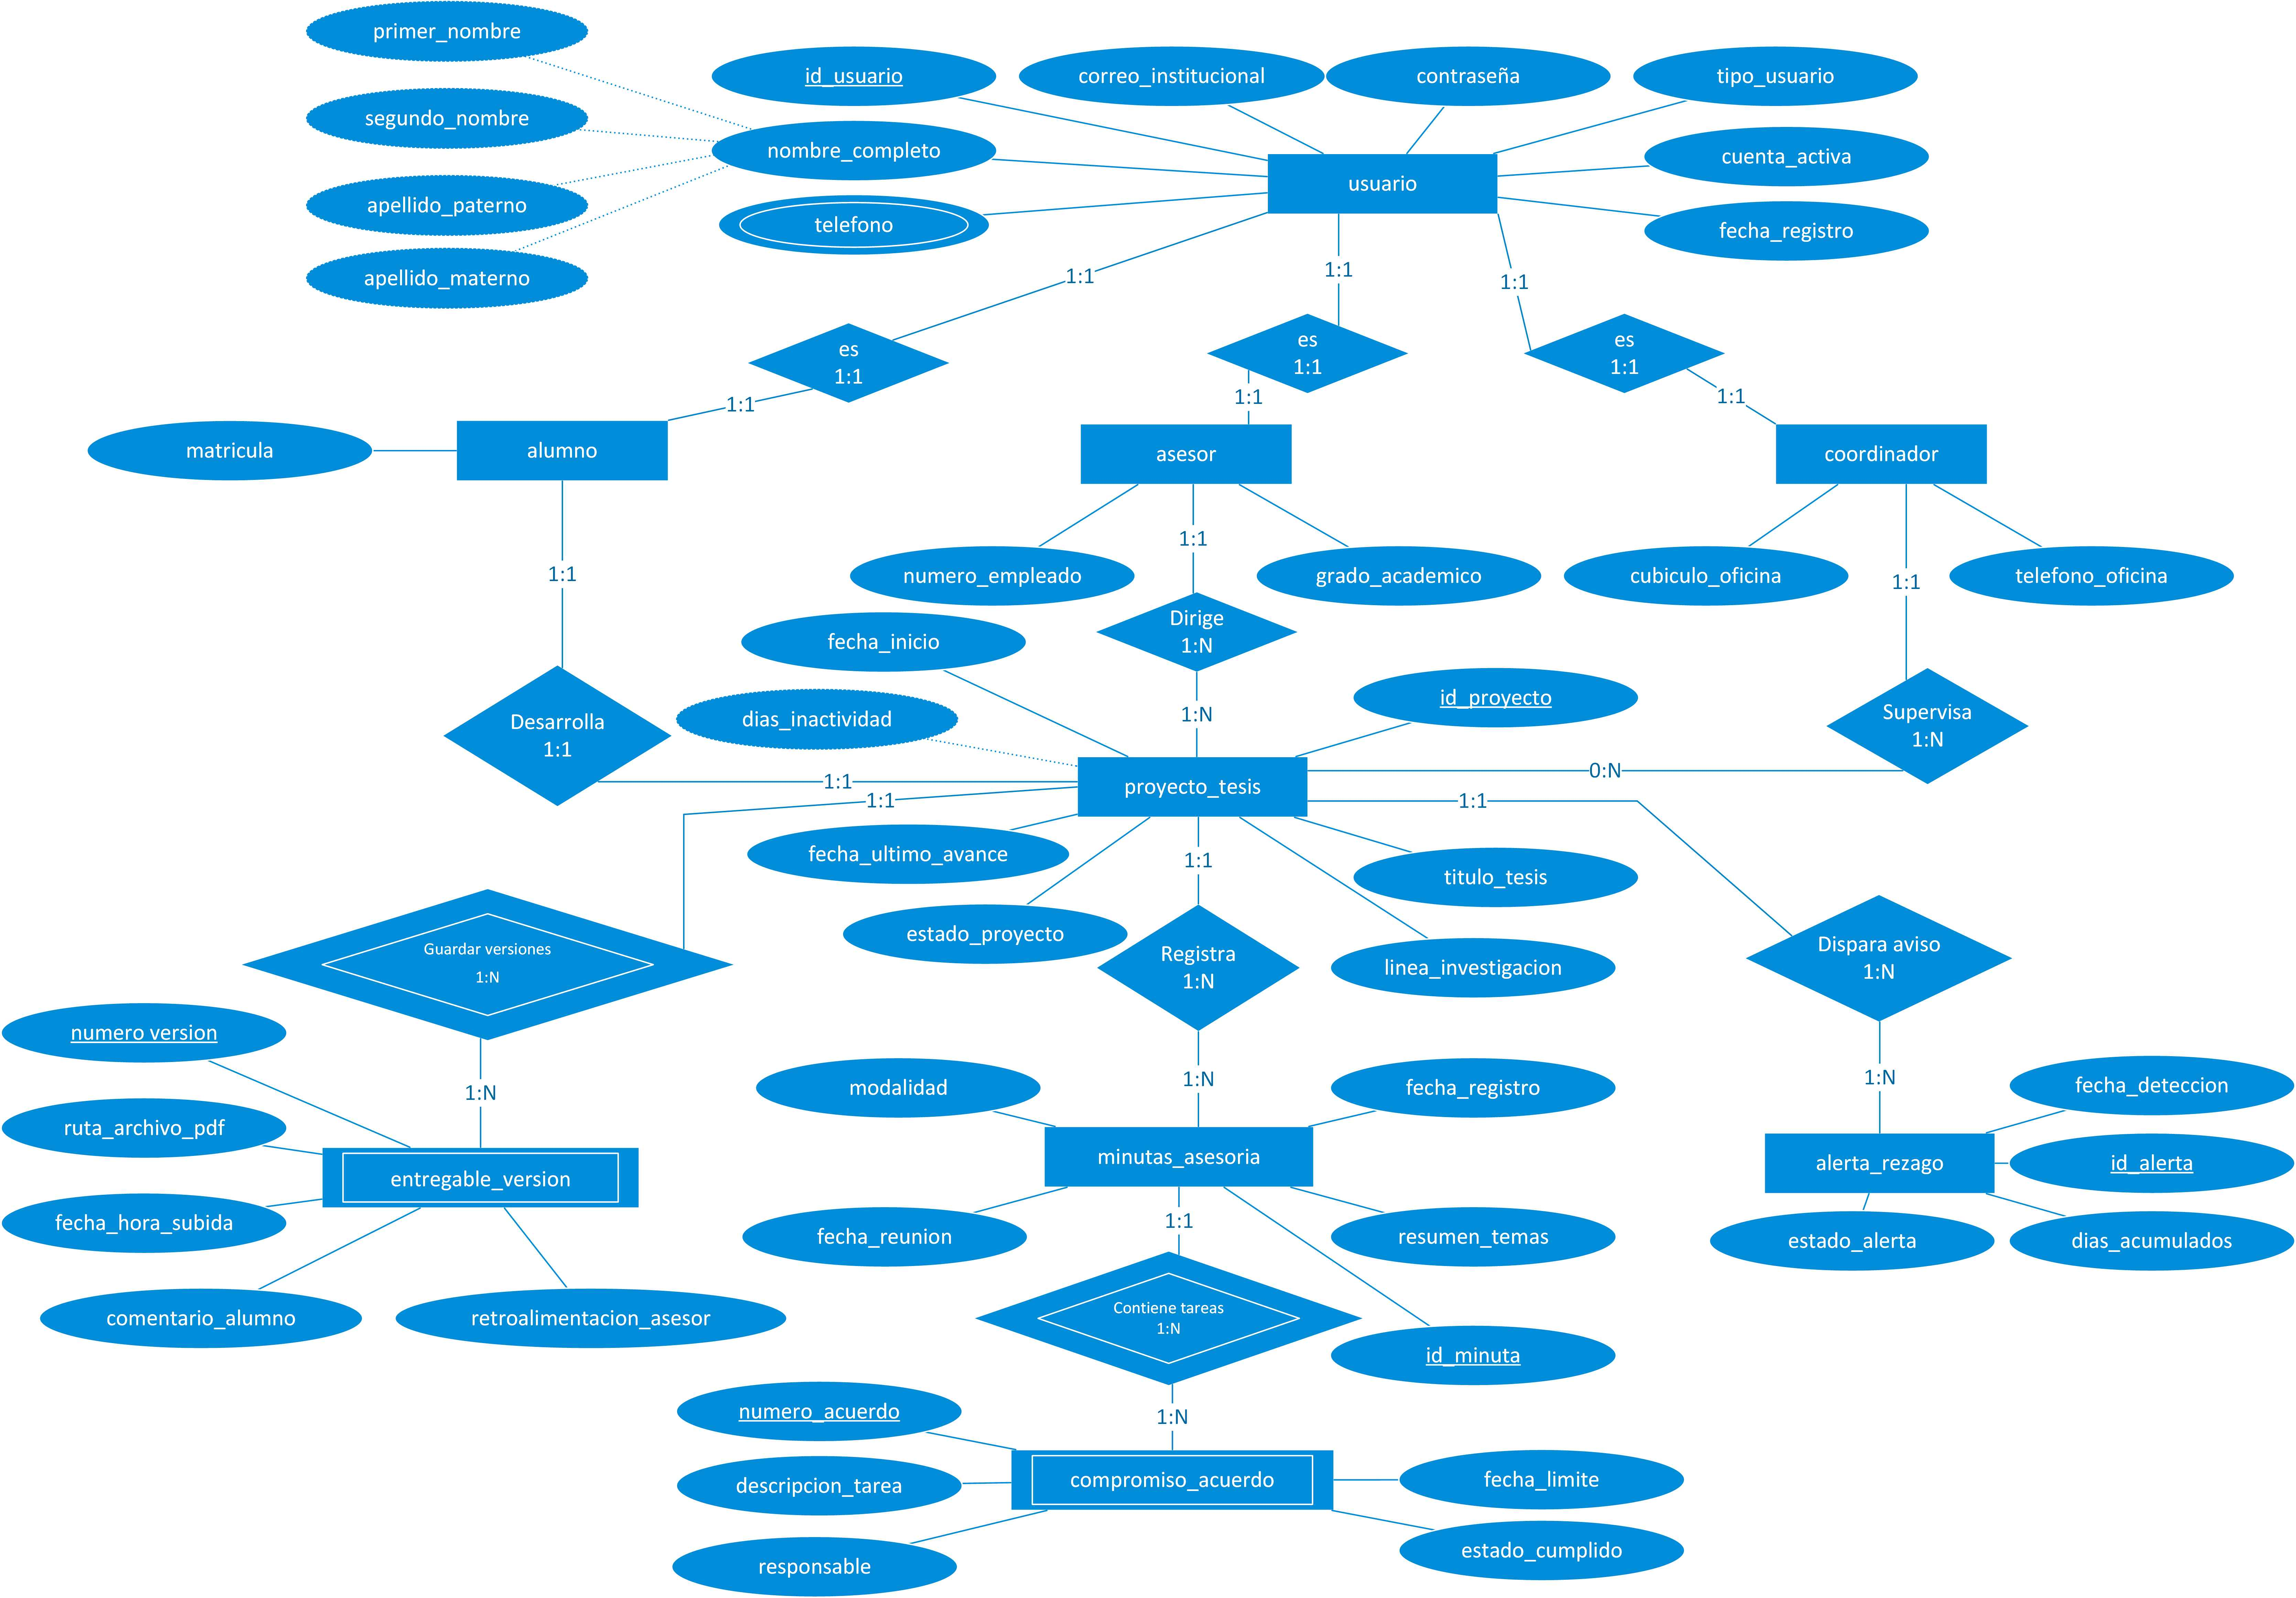
\includegraphics[width=1\linewidth]{assets/database/db-MER.jpg}
    \caption{Diagrama Entidad--Relación Extendido de la página web para seguimiento de tesis.}
    \label{fig:diagrama_eer}
\end{figure}